The SAM Mark I includes every system that is compulsory in order to satisfy the given requirements meanwhile optimizing the aircraft's safety, and comfort. The aircraft's main systems are flight controls, deicing systems, engine control systems, environmental control systems, fuel systems, battery systems, along with an electrical and hydraulic system. These systems were chosen to provide the aircraft with the latest system technologies that are not present in older aircraft, and to provide safe flights. Due to the fact that the SAM Mark I is a large aircraft, each system has a redundancy factor built into it in case of a malfunction of any part. 

\subsection{Flight Controls}
The SAM Mark I will utilize a Fly-By-Wire (FBW) flight control system in order to help reduce overall airframe weight and increase the ease of maintenance and manufacturing, and increase the complexity of the controls. A typical conventional primary flight control system on an aircraft incorporates hydraulic actuators and control valves, that are controlled by pilot driven cables \cite{fbw}. Due to the long cable runs, however, this conventional system adds to the overall system weight and increases the amount of total components in the system, which is why the electronic based FBW system was chosen for the SAM Mark I. The FBW system relies on electronic computers that are located in the cockpit’s main flight control computer. Position transducers are attached to pilot controls which send electrical signals for the computers to convert into commands that are then communicated to the actuators \cite{fbw}. The SAM Mark I will also include a secondary electric computer in case the main flight computer breaks down or fails to send the required signals, and a secondary FBW system in case of main system failure.

The primary flight controls included in the SAM Mark I are: one outboard aileron, multiple flaperons and spoilers per wing, an elevator per horizontal stabilizer wing, and a single rudder on the vertical horizontal tail. These control surfaces on the wings and tail are operated by hydraulically powered, electrically signaled actuators. Each elevator, flaperon and aileron surface will be controlled by two actuators, while the vertical tail rudder will be controlled by three. These control surfaces that will be controlled by the fly-by-wire system will improve the SAM Mark I’s system reliability and maintainability.

\begin{figure}[H]
    \centering
    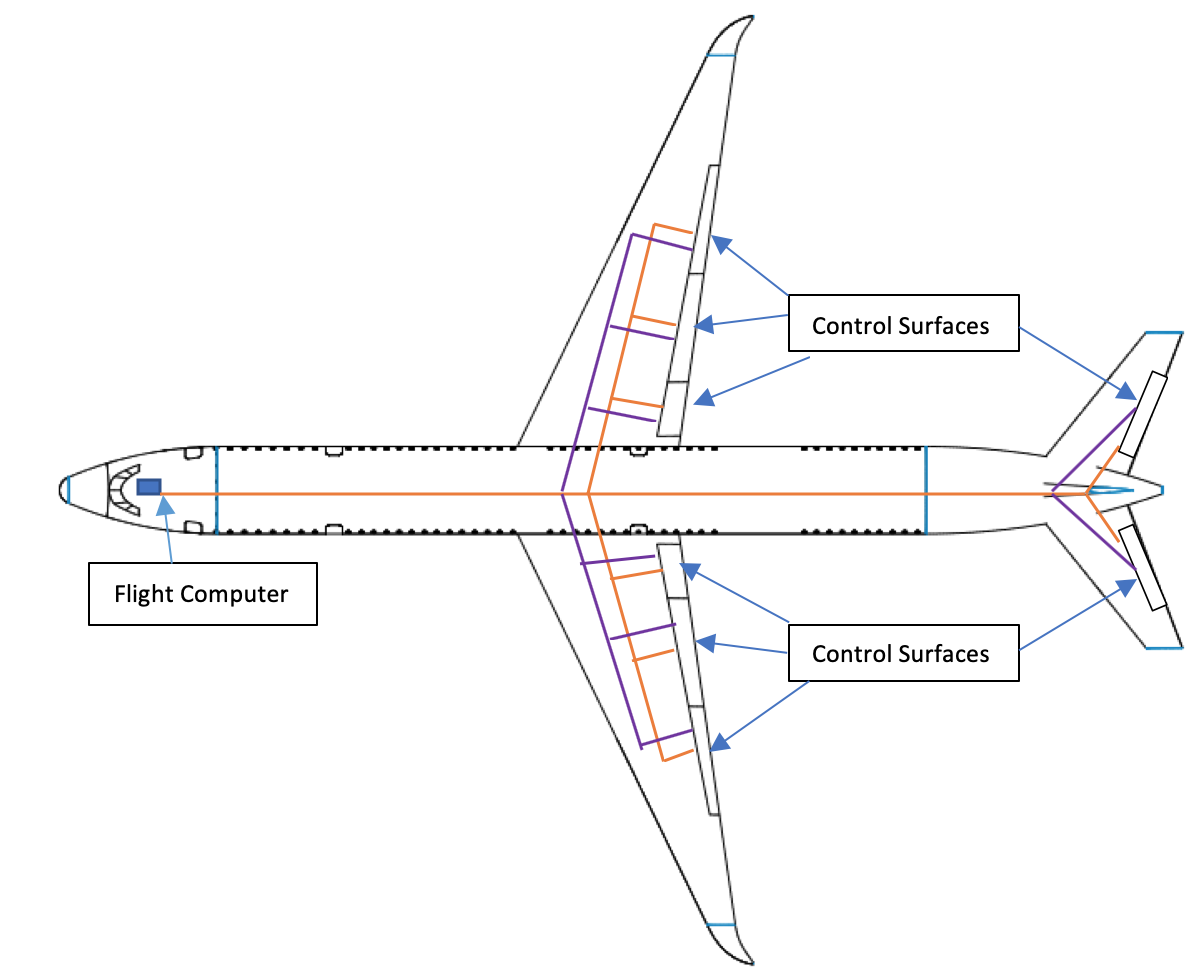
\includegraphics[width=.75\linewidth]{Photos/systems/flight_controls.png}
    \caption{Flight Controls Diagram}
    \label{flighte_controls}
\end{figure}

\subsection{Engine Controls}
The SAM Mark I will utilize a full authority digital engine control (FADEC), which will contain an engine control unit (ECU) and all components related to maintaining quality engine performance. The ECU's will be located on the engine's fan casing. The FADEC system was chosen because it provides the aircraft with optimum engine efficiency. The ECU within the FADEC system receives a variety of input data such as air density, engine pressure and throttle position, and after analyzing it, relays the information to FADEC which then computes the necessary engine parameters such as fuel flow, or air bleed valve position. The FADEC system is also responsible for engine starting and restarting, and during flight, applies calculated engine settings by sending electrical signals to the GE90-115B engines on the SAM Mark I. The one drawback to the FADEC system, however, is its inability to be overridden manually, meaning that the computer will have full control of all parameters of the engine. Although the automation of engine controls provides no room for human error during flight, if the FADEC system were to fail, all engines would fail as well. Therefore, a manual override will be installed in the cockpit capable of putting the aircraft's engines into manual mode in case the FADEC system experiences failure.  

\begin{figure}[H]
    \centering
    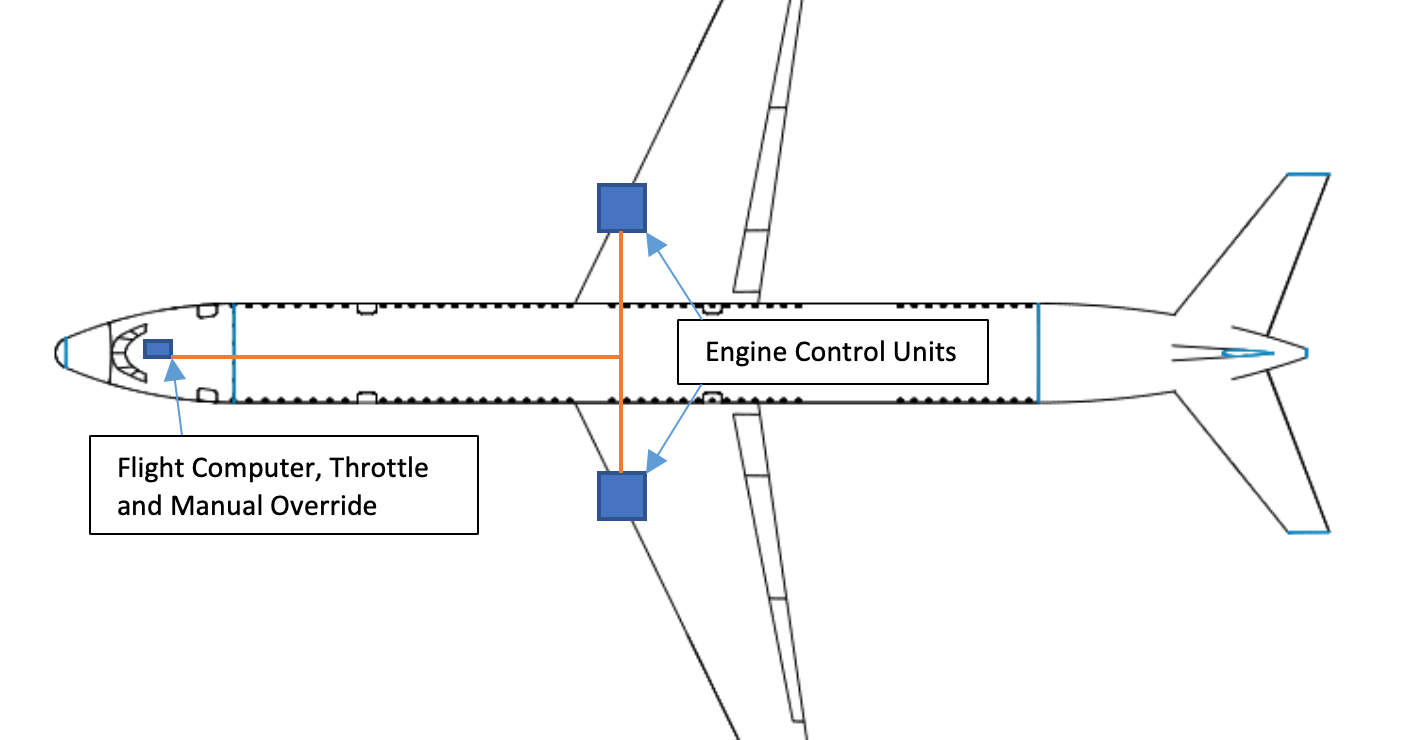
\includegraphics[width=.85\linewidth]{Photos/systems/engine_controls.png}
    \caption{Engine Controls Diagram}
    \label{engine_controls}
\end{figure}

\subsection{Fuel System}
The SAM Mark I’s fuel system is designed to effectively and safely feed the aircraft’s engines during flight. The SAM Mark I will store fuel two tanks; one in the left wing, and one in the right wing, since the designed wings can hold more fuel than the SAM Mark I requires. Each fuel tank will contain two fuel boost pumps in order to supply the engine with fuel. This fuel system will also incorporate the use of the fuel quantity indicating system (FQIS) which is made up of ultrasonic sensors throughout the tanks. These sensors send signals to a processor which calculates the volume, density, and mass of the fuel, allowing the FQIS to determine the current amount of fuel in the tank, and take control of refueling commands for each fuel tank \cite{fuel_system}. Furthermore, the FQIS system is also responsible for maintaining the correct amount of fuel in each tank, and shutting off re-fuel valves when a fuel tank reaches its designated volume. Figure \ref{fuel_tank} demonstrates the placement of fuel tanks aboard the SAM Mark I with their connected fuel lines, and the FQIS system that sends fuel data back to the cockpit.

\begin{figure}[H]
    \centering
    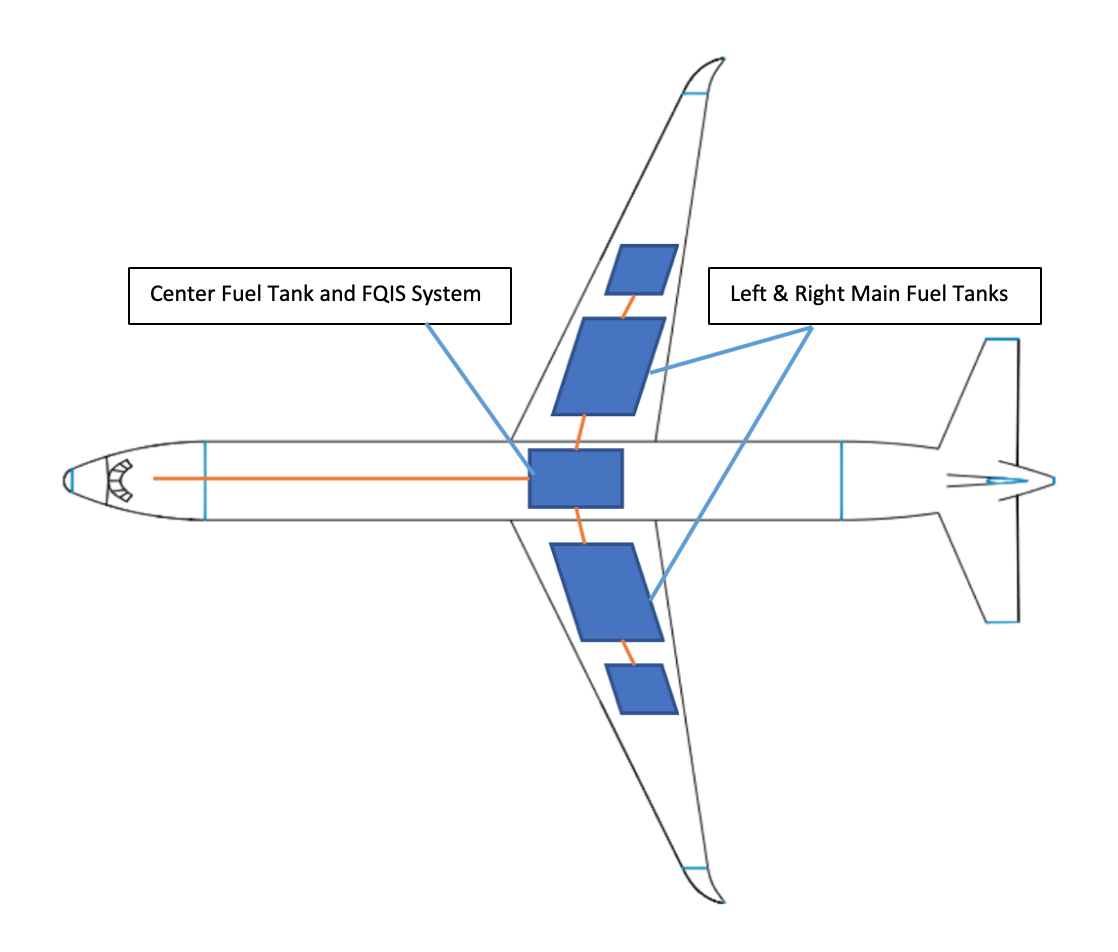
\includegraphics[width=.85\linewidth]{Photos/Fuel_tanks.png}
    \caption{Fuel System Diagram}
    \label{fuel_tank}
\end{figure}
 
\subsection{Hydraulic System}
The SAM Mark I will incorporate three hydraulic reservoirs as part of its hydraulics system. Each reservoir contains hydraulic fluid that is used to control the flap systems, actuators, brakes, landing gear, and thrust reversers. Since the SAM Mark I utilizes a fly-by-wire flight control system, the aircraft’s hydraulic system will only be used to operate control surfaces. Each reservoir will also contain an engine-driven pump (EDP) which provides hydraulic power to the system and transfers hydraulic fluid to each control surface. As a backup system, each reservoir will also contain secondary motor-pumps in case of failure of the EDPs. The left and right hydraulic systems will each control their respective thrust reversers, along with each side’s respective ailerons, flaperons and elevators. The main center hydraulic system will supply pressurized hydraulic fluid in order to control the normal brake system, nose landing gear actuation and steering along with the main landing gear actuation and steering. Each hydraulic system will also have an indication system that consists of hydraulic sensors that measure and send the hydraulic pressure and temperature to the main flight computer. A detailed diagram of the SAM Mark I’s hydraulic system is presented in Figure \ref{hydrualics}. 

\begin{figure}[H]
    \centering
    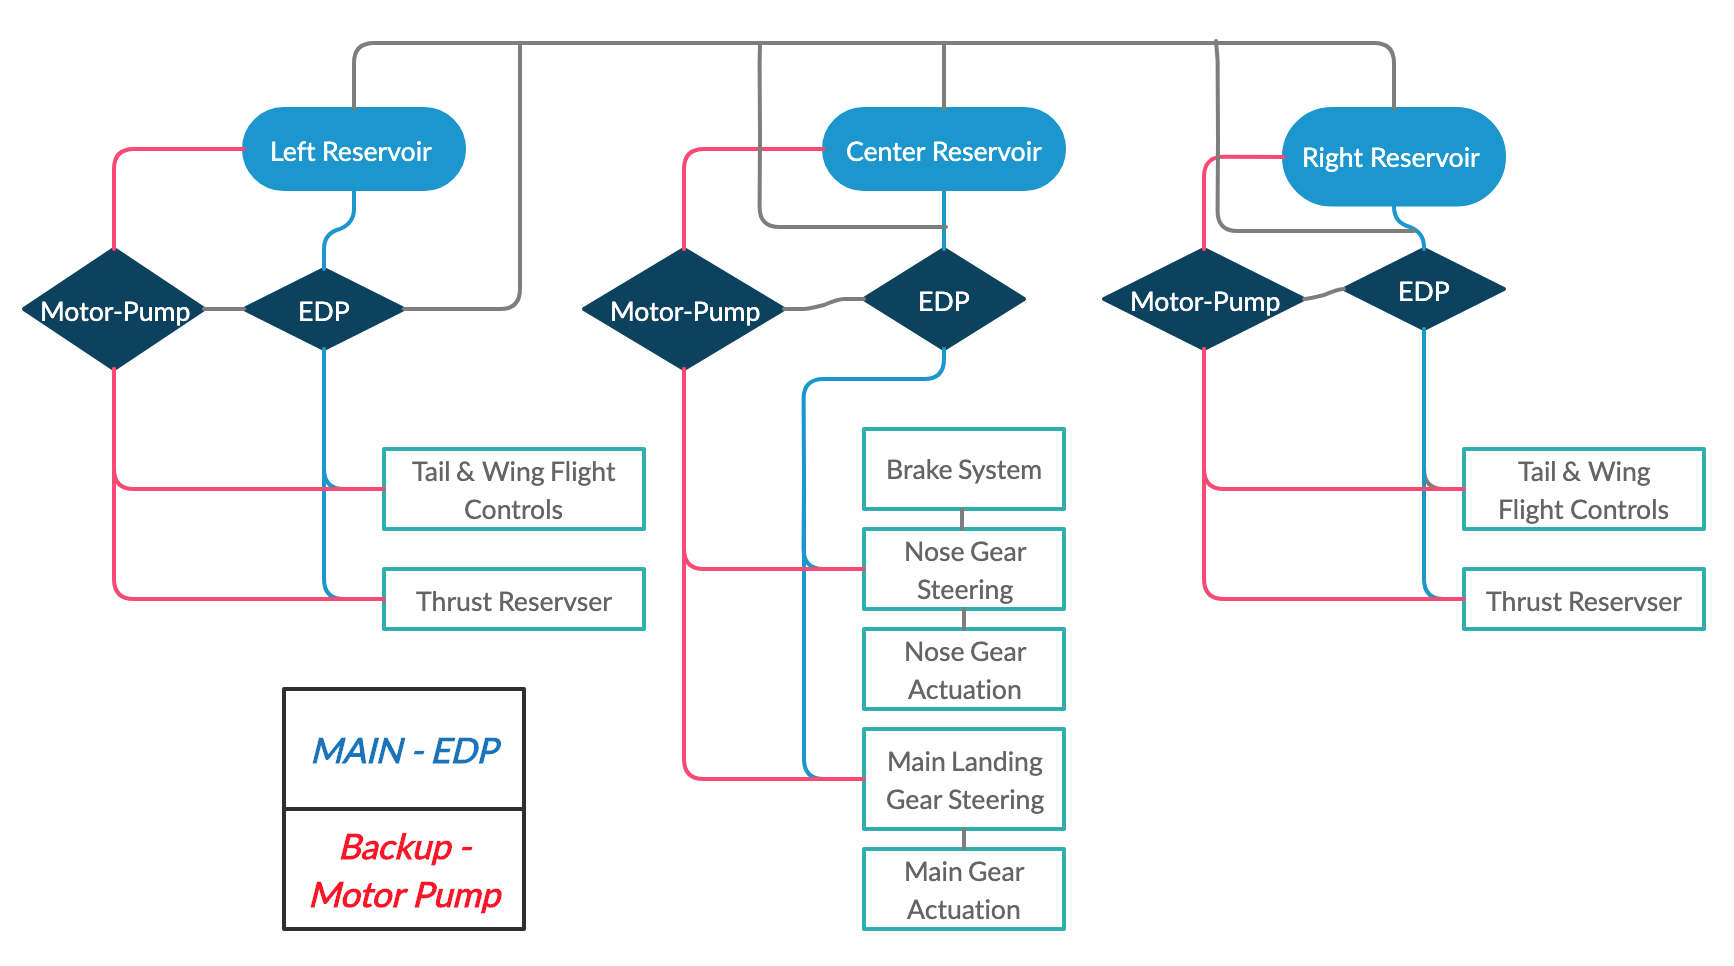
\includegraphics[width=.85\linewidth]{Photos/systems/Hydrualics.png}
    \caption{Hydraulic System Diagram}
    \label{hydrualics}
\end{figure}

\subsection{Electrical System}
Since the SAM Mark I is a large, multi-engine aircraft, it will contain two independent electrical systems: one main and one backup system. The main electrical system will consist of a generator located on each engine, a generator that is run by an auxiliary power unit (APU), three generator control units, one for each generator, and a bus power control unit. Three generators are included in this aircraft, one on each engine, and one on the APU, in order to share electrical loads and provide redundancy. Each of the main generators has the ability to serve either of one or both of the two main busses. The generator control units serve the purpose of regulating voltage and controlling frequency throughout the electrical systems \cite{electrical_system}. The bus power control unit is used to help the SAM Mark I distribute electrical power between the different busses on the aircraft. Two batteries will be included in the aircraft as well for powering the starting and backup systems. The backup electrical system also includes two engine-driven generators in case the main generators fail. Furthermore, each engine generator contains an integrated drive generator (IDG) which allows the drive to operate at constant speed \cite{electrical_system}. Each IDG also contains a generator circuit breaker which allows for the engine to operate its respective bus, and the two main busses are connected by a bus tie breaker. The bus tie breakers provide redundancy in case one of the IDGs fails, allowing the other engine IDG to power both busses. A detailed schematic of the electrical system is demonstrated in Figure \ref{electrical_system}. 

\begin{figure}[H]
    \centering
    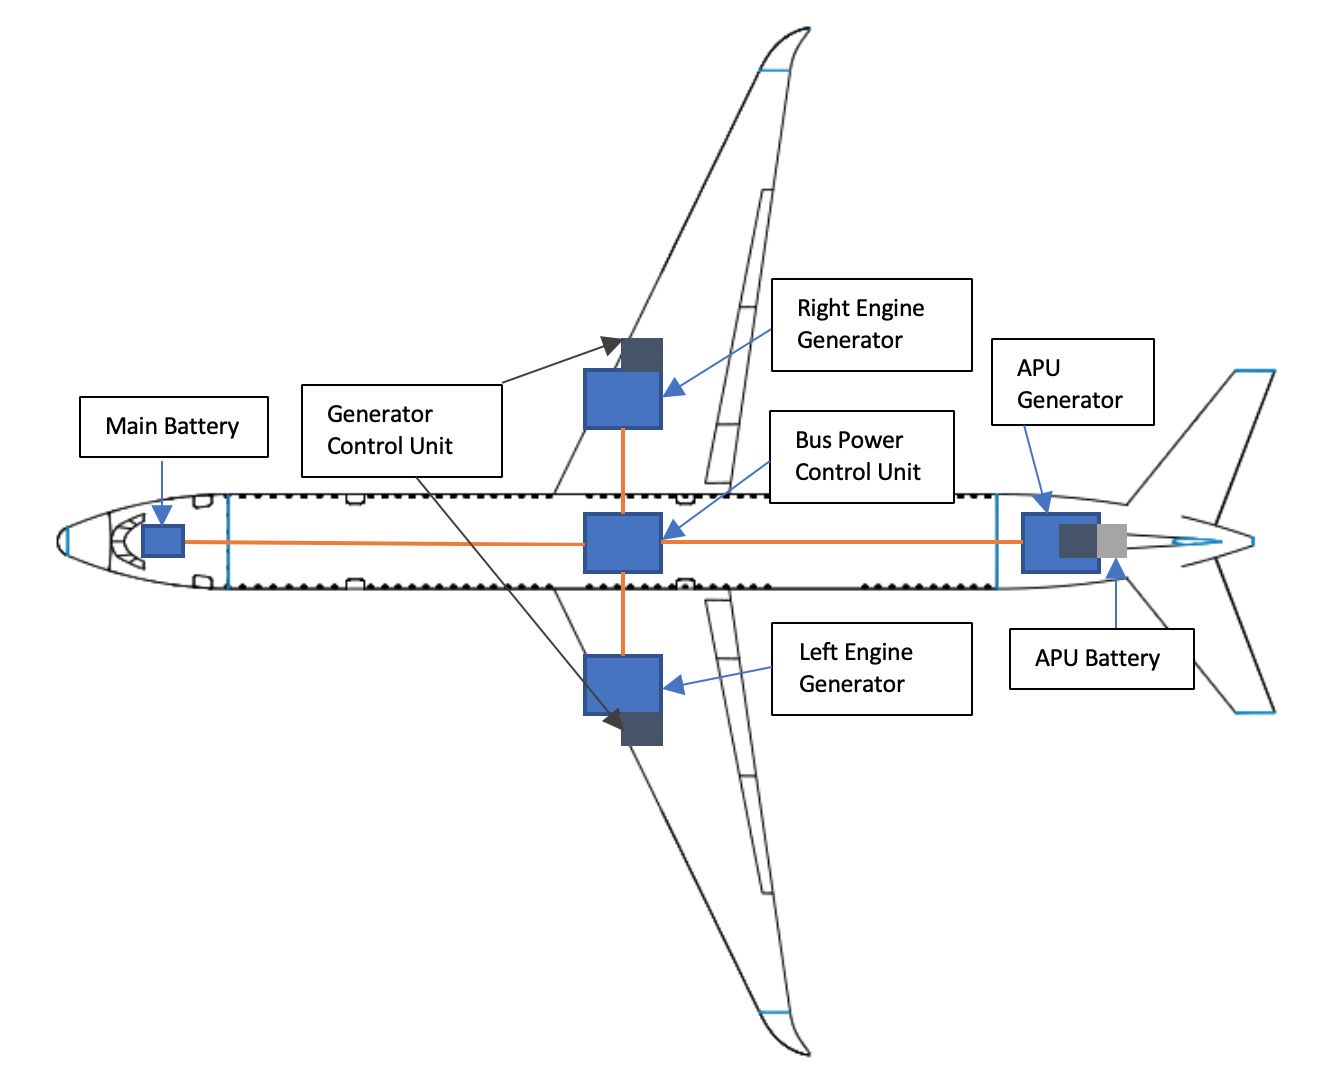
\includegraphics[width=.75\linewidth]{Photos/systems/electrical_system.png}
    \caption{Electrical System Diagram}
    \label{electrical_system}
\end{figure}


\subsection{Pneumatic and Environmental Control System}
The SAM Mark I will incorporate an environmental control system in order to provide a comfortable flight experience for all passengers. The aircraft will contain an air conditioning and heating system that will regulate the air temperature throughout the cabin. The aircraft will contain an environmental control unit (ENCU) that will obtain compressed air from the compressor stages of the engines during flight. Inside the ENCU, the air is further compressed to the correct pressure and temperature conditions and excess moisture is removed \cite{env_system}. After the air is conditioned, it is distributed throughout the aircraft at the desired temperature and pressure. Due to the 39,000 ft cruise flight, The SAM Mark I will also contain a pressurization system in order to set the cabin pressure to 8,000 ft pressure altitude at maximum flight altitude. The pressure will be maintained by two out-flow valves located on the aircraft, which will be opened sparingly throughout flight to prevent the fuselage from under or over pressurizing. The SAM Mark I will also contain a pneumatic bleed air system to prevent ice from forming on the aircraft’s surfaces including the wings, tail and control surfaces. The bleed air is collected from the aircraft jet engine’s compression stage, where it is then distributed to the wings, tails, and engine inlets through a series of piccolo tubes. These tubes then connect to holes located under the surfaces of the wings and control surfaces, where the hot bled air is then dispersed. This system allows the surfaces to stay above freezing temperature, and prevents ice from changing the shape of the wing, which leads to a decrease in performance.

\subsection{Emergency System(s)}
There will be a main emergency system put into place in the SAM Mark I that will focus on prevention of accidents and the protection of the passengers. The main flight computer will have the standard alarm and warning systems designated to notify the pilot of any problems the aircraft is experiencing. Fire detectors will be placed throughout the aircraft, and a fire extinguisher will be located in the cabin and rear of the aircraft. Under each seat there will be emergency life vests, and emergency oxygen masks will be stored in compartments above each passenger and crew seat. There will also be eight emergency exits on the aircraft, each immediately deploying evacuation slides in case of a crash landing. 

\subsection{Avionics (JJ)}
\subsubsection{Integrated Avionics System}
In order to determine which manufacturer and system provided the most holistic, yet economical avionics suite for the SAM Mark I, a comprehensive trade study was assessed on many contemporary civilian and military aircraft, as well as the updated systems offered for legacy aircraft.  Predominantly military aircraft were included because of their shared platform (tankers, reconnaissance) with older jetliners, as well as their perceived weight and cost savings at the minor expense of elegance: key for one of the most expensive aspects budget-driven design. 

\begin{table}[!h] 
    \centering
    \caption{IAS Usage Throughout Industry}
    \begin{tabular}{ |c||c|c|c|c|c|}\toprule
    \textbf{Aircraft}  & Boeing 787 & Boeing 777 & Boeing 767/757 (Update) & Airbus A220 \\\hline 
    \textbf{IAS Provider} & General Electric & Honeywell & Rockwell Collins & Rockwell Collins  \\\hline
    \textbf{IAS System} & Common Core & AIMS & Flight2 & Pro Line Fusion \\\hline \hline
    \textbf{Aircraft}  & Lockheed C-130 & Boeing E-3 (707) & Northrop Grumman E-8 & Boeing KC-135 (707) \\\hline
    \textbf{IAS Provider} & Rockwell Collins & Rockwell Collins & Rockwell Collins & Rockwell Collins  \\\hline
    \textbf{IAS System} & Flight2 & Flight2 & Flight2 & Flight2
    \\ \bottomrule
    \end{tabular}\label{tab:ias}
\end{table}

From this study, the above (Table \ref{tab:ias}) three manufacturers and their respective integrated avionics systems (IAS) stood out as candidate systems for SAM Mark I.  To further adjudicate between, the accompanying flight control (autopilot) systems (FCS) capable of running parallel or integral to the IAS were analyzed, with Rockwell Collins' Flight2 system standing out due to the steadfast integration of a comprehensive, proven FAA-approved and certifiable FCS \cite{fcs7000pdf}.  Additionally, the military-derived simple flight deck \cite{flight2page} offered simple, rugged, ambient-air-cooled avionics \cite{flight2pdf} without the associated cost or weight of the large-format type displays found in the latest commercial aircraft \cite{flight2page}.  The IAS system will be stowed within the Electronics $\&$ Engineering (E $\&$ E) bay beneath the forward galley, where there is easy access to electrical power and the cockpit.  Requiring no external cooling or other special considerations, installation should not be difficult.  Flight2 is also compatible with upgraded (all glass, large format) flight decks at carrier discretion \cite{flight2page}. 


\subsubsection{Flight Control System}
The latest RC Flight2 IAS features digital autopilot built off legacy systems which have been extensively proven through two decades of military and civilian use \cite{flight2page}.  RC's FCS-7000 is a complete FCS with a host of capabilities \cite{fcs7000pdf} including:

\begin{itemize}
    \item Fail passive, independently selectable dual autopilot computers capable of:
        \begin{itemize}
            \item IFR and VFR Flight
            \item Takeoff (selected from control yoke on ground)
            \item Go around (selected from control yoke in air)
            \item Pitch attitude hold
            \item Altitude hold (Reduced vertical separation minimum (RVSM) compliant)
            \item Altitude preselect (RVSM compliant)
            \item Flight level change (airspeed/mach/vertical speed selection)
            \item Vertical navigation (VNAV) (coupled to FMS) – RVSM compliant/altitude modes
            \item Terrain Following/Terrain Avoidance-growth
            \item Approach (Very High Frequency (VHF) Omni-Directional Range (VOR), ILS, Microwave Landing System (MLS), Global Positioning System (GPS) Localizer performance with vertical guidance (LPV))
            \item Pitch sync
        \end{itemize}
    \item Category II (Category IIIA capable) instrument landing
    \item Required Navigation Performance (RNP) RNAV 0.10, LPV (with GPS Wide Area Augmentation System (WAAS)) precision approaches
    \item FMS coupled VNAV for coupled climb, cruise, descent and approach performance/fuel optimization
    \item Gloved hand operation
    \item Flexible FD human-machine interface tailored to desired carrier systems
    \item Accommodation of a wide range of digital sensors, including display systems, as optioned by carriers
    \item FAA approved (TSO-C9c) and FAR part 23 and 25 certifiable, with design assurance level A (flight critical safety)
    \item 20-year guaranteed non-obsolescence
\end{itemize}

The decision to option an advanced FCS, significantly exceeding the AIAA RFP \cite{RFP} mandated requirements, was not taken lightly given the otherwise conservative and budget-centric nature of this aircraft. However, Toucan Aviation can not and will not discount the unequalable responsibility for the safety and well being of over 410 unique lives dependant upon the SAM Mark I for safe flight in all conditions.  Carriers will retain the option to work with RC to certify legacy Flight2-compatible autopilot systems with the FAA upon delivery.   

\subsubsection{Additional Avionics Hardware and Systems}

A holistic avionics system requires many subsystems and pieces of hardware assembled from a plethora of suppliers.  Those are outlined in a preliminary overview fashion on a supplier basis below, in \ref{tab:hardware} and \ref{tab:software}, which reference the additional hardware and software systems, respectfully.  The baseline for these systems can be traced to the original comparison/trade study \ref{subsection: comparison} analysis winner: Boeing's 777-200 \cite{suppliers}.

\begin{table}[!h]
\centering
\caption{Supplemental Avionics Hardware by Supplier}
\begin{tabular}{|l|l|}
\hline
\textbf{Supplier}                   & \textbf{Item(s)}                                                                                                                                                                                                                                                         \\ \hline \hline
ACSS                                & NXT-800 Mode S transponder                                                                                                                                                                                                                                                           \\ \hline
AstroNova INC                       & \begin{tabular}[c]{@{}l@{}}ToughWriter 5 flight deck printer\\ Cabin printer(s)\end{tabular}                                                                                                                                                                                         \\ \hline
AvtechTyee                          & Onboard intercom                                                                                                                                                                                                                                                                     \\ \hline
CMC Electronics, INC                & CMA-2102SB Satcom high gain antenna system                                                                                                                                                                                                                                           \\ \hline
Collins Aerospace                   & \begin{tabular}[c]{@{}l@{}}AOA indicators\\ AOA sensors\\ Flow sensors\\ Ice-detection sensors\\ Pitot/static probes\\ (Total) air-temperature sensors\\ MultiScan ThreatTrack weather radar\\ External \& Taxi Aid Camera System\\ Proximity sensor data concentrators\end{tabular} \\ \hline

Harris Antenna Products & VHF communication antennas                                                                                                                                                                                                                                                           \\ \hline
Honeywell Aerospace                 & \begin{tabular}[c]{@{}l@{}}Multi-mode receivers\\ IntuVue advanced weather radar\\ Satellite Communications (SATCOM) high speed digital voice \& data communications\end{tabular}                                                                                                    \\ \hline
Moog Controls                       & Primary flight controls                                                                                                                                                                                                                                                              \\ \hline
Safran Aerosystems                  & Illuminated cockpit panels                                                                                                                                                                                                                                                           \\ \hline
Systron Donner Inertial             & Inertial Measurement Unit (IMU) for Rockwell Collins flight control module                                                                                                                                                                                                           \\ \hline
Thales Avionics                     & Large format cockpit \& cabin printers                                                                                                                                                                                                                                               \\ \hline
QED, INC                            & Bourdon tube pressure gauges, pressure switches and pressure gauge/switch combinations                                                                                                                                                                                               \\ \hline
\end{tabular} \label{tab:hardware}
\end{table}

\begin{table}[!h]
\caption{Supplemental Avionics Systems/Software by Supplier}
\centering
\begin{tabular}{|l|l|}
\hline
\textbf{Supplier}   & \textbf{Item(s)}                                                                                                                                       \\ \hline \hline
Collins Aerospace   & External \& Taxi Aid Camera System                                                                                                                     \\ \hline
Honeywell Aerospace & \begin{tabular}[c]{@{}l@{}}Traffic/Aircraft Alert and Collision Avoidance System (TCAS/ACAS)\\ Air Data Inertial Reference System (ADIRS)\end{tabular} \\ \hline
\end{tabular} \label{tab:software}
\end{table}

\subsubsection{Fitment and Layout}
The majority of the Avionics system outside of the cockpit will be stowed beneath the forward galley \hl{cite KP} in the E $\&$ E bay.  Fortunately, due to both this aircraft's large barrel diameter and the relatively low pressure for cargo, there is a significant amount of available space beneath the flight deck for the placement of subsystems.  \hl{elaborate on size and fitment}  

\subsection{Certs that may apply}

\texthl{25.831 Ventilation - Designed to provide each occupant with an airflow containing at least 0.55 pounds of fresh air per minute}
\texthl{}

\clearpage
% \textcolor{red}{
% Discuss the follow subsystems. Each should include specifications, justifications, and
% configuration inside the aircraft as applicable. These auxiliary systems should integrate
% appropriately with other aircraft systems.
% o Flight Controls
% o Engine Controls
% o Fuel System
% o Hydraulics System
% o Electric System
% o Pneumatic System
% o Environmental Control System
% o Emergency System(s)
% o Avionics (Navigation \& Communication)}